
\subsection{Move IIIb}
Let $A^\pm = A = \Z_2\<{a,b,c, a_1, ..., a_l}$ where $a,b$ and $c$ are as shown in
figure \ref{fig:move_iiib} and again $a_1,...,a_l$ denote the crossing outside a
neighbourhood of where the bifurcation occur. Again, the grading of
$a,b$ and $c$ is unchanged and thus $A^+$ and $A^-$ are isomorphic as graded
vector spaces.

\figpdf{.6}{move_iiib}{.}

Let $f_\pm \in \tilde{W}_3(Y)$ be the immersion whose images are the small
triangles $T_\pm$ with vertices $a,b,c$, then by lemma
\pref{prop:deg_sum}, we find that $\deg(a) = \deg(bc)$.

Let $g: TA \to A$, such that $g_2(b,c) = a$, $g_1 = \id_A$
and $g$ is otherwise zero. Then $g^2 = g \circ g = \id^A$, since 
\[ g^2(b,c) = g_2(g_1(b),g_1(c)) + g_1(g_2(b,c)) = a+a = 0, \]
and we claim, 
\begin{equation}
\label{eq:move_iii_a_inf_rel}
\sum_{r,s,t} g_u(\I^{\otimes r} \otimes m^+_s \otimes \I^{\otimes t}) 
= m^-_n \circ g 
% \quad \qty( := \sum_{i_1,...i_r} m^-_r (g_{i_1} \otimes g_{i_2} \otimes ... \otimes g_{i_r}) ) .
\end{equation}
So $g$ is a tame \Ainf-isomorphism from $(A, m^+)$ to $(A,m^-)$.

\begin{remark}
In addition to \pref{eq:move_iii_a_inf_rel}, we also requite that the equation
with plus and minus swapped is satisfied. Since this is the condition for $g =
g^{-1}: (A, m^+) \to (A,m^-)$, to be an \Ainf-homomorphism. 
However, this follows immediately, by the symmetry of the problem when
reversing the direction of time.
\end{remark}

\lskip
Consider $f \in W^+_k(Y_{t'\pm \epsilon})$, then the triangle $T_\pm$ cannot be
the image of $f$, since it a two positive vertices. Assume $f$ maps an edge
$X_i$ of $\Pi_k$ to one of the sides of $T_\pm$. Then a
neighbourhood of $X_i$ is mapped to one of the shaded areas in
\pref{fig:move_iiib}. If the shaded area is marked with (1) or (2), clearly $f
\in W^+_k(\Ypm,a)$ (ie. $f(x^k_0) = a$,) since $a$ is positive. 

\begin{lemma}
If the shaded area marked by (3), $f(x^k_0) = a_i$ for some $i \in
\{1,...,l\}$.
\end{lemma}

\begin{proof}
Indeed, by corollary \pref{prop:height_sum}, $f(x^k_0) \ne
f(x^k_i)$ for $i\ne0$, so $f(x^k_0)$ cannot be $b$ nor $c$. 
Also if $f(x^k_0) = a$, then by lemma \pref{prop:l_6.1}, 
\[ H(a) - H(b) - H(c) > |f(\Pi_k)| > 0. \]
However, by applying lemma \pref{prop:l_6.1} to the $f_\pm$, 
$H(b) + H(c) - H(a) = |T_\pm| > 0$.
\end{proof}

In order to prove the claim \pref{eq:move_iii_a_inf_rel} we will simplify
the problem, by fixing a generator $v \in \Cc$ and consider the problem
restricted to the one-dimensional subspace spanned by $v$. ie. 
\begin{equation}
\label{eq:move_iii_a_inf_rel_pr}
\pr_v \circ \left\{ \sum_{r,s,t} g_u(\I^{\otimes r} \otimes m^+_s \otimes \I^{\otimes t})
\right\} = \pr_v \circ\:  m^-_n \circ g . 
%
%= \pr_v \left\{ \sum_{i_1,...,i_r} m^-_r (g_{i_1} \otimes g_{i_2} \otimes ... \otimes g_{i_r}) \right\}.  
\end{equation}



\subsubsection{Case $v \ne a$:}
First, we'll assume $v \ne a$. Then by the definition of $g_n$, 
$\pr_v \circ \: g_n = 0$ if $n\ne 1$ and $g_1 = \id_A$, so the left hand side of the equation
simplifies to $\pr_v \circ\: m^+_n$. 

To prove this equation, there are 6 different kinds of fragments, we
need to consider (Numbered $a_\pm, b_\pm$ and $c_\pm$ in figure
\pref{fig:move_iiib1} ).

\figpdf{.8}{move_iiib1}{.}

\newcommand{\tA}{\tilde{A}}
\newcommand{\tC}{\tilde{\Cc}}
\newcommand{\tm}{\tilde{m}}

It turns out that the terms in $m^\pm$ coming from fragments that look like
$a_\pm$ transforms differently form terms coming from $b_\pm$. In order to
distinguish between these two cases we will define a new vectors space
$\tA = \Z_2\<{a',a'',b,c,a_1,...,a_l}$ and a family of maps
\[ \tm^\pm_k : \tA^{\otimes k} \to \tA.  \]
(Note that we will not require that the maps satisfy the \Ainf relations.)
Let $\tC = \{ a',a'',b,c,a_1,...,a_l\}$ denote the set of generators.

Like in section \pref{sect:Ainf_m}, let $v_1,...,v_k \in \tC$ and 
\[ \tilde{\M}^v_{v_1,...,v_k}(Y_{t'\pm\epsilon}) = \{ u \in W^+_k (Y_{t'\pm\epsilon},v) \q| u(x^k_i) = v_i \}, \]
where by $u(x^k_i) = a'$ (resp. $u(x^k_i) = a''$), we means that $u(x^k_i) = a$
and a neighbourhood of $x^k_i$ in $\Pi_k$ is mapped to the shaded area in
\pref{fig:move_iiib1}, marked by $a_\pm$ (resp. $b_\pm$). For $v_1,...,v_k \in \tC$, define 
\[ \tm^\pm_k(v_1,...,v_k) = \sum_{v\in\tC} (\#_2
\tilde{\M}^v_{v_1,...,v_k}(Y_{t'\pm\epsilon})) v. \]

Define $\sigma : TA \to \tA$, by $\sigma_1(v) = v$ for all 
$v\in \{ b,c,a_1,...,a_n \}$, \[  \sigma_1(a) = a' + a'' \] and $\sigma_k = 0$ for
$k>1$. Also define $g', g'': T\tA \to \tA$, by 
\[ g'_1 = g''_1 = \id_{\tA}, \quad g'_2(b,c) = a', \quad g''_2(b,c) = a''  \]
and both are otherwise 0. Since $(\tA,m^\pm)$, is not an \Ainf-algebra,
it make non sense to speak of these maps as \Ainf-homomorphisms. However we
can still, consider their composition like definition \pref{def:Ainf_comp}.
Then it is quite easy to check that 
\begin{equation}
\label{eq:sigma_g}
\sigma \circ g = g' \circ g'' \circ \sigma 
\qq\tand
\pr_v \circ\: m^- = \pr_v \circ\: \tm^m \circ\: \sigma. 
\end{equation}

\newcommand{\bm}{\overline{m}}

We will define two  more families of maps $\bm_k: A^{\otimes k} \to A$. 
Consider the subset $S_\pm(v) \subset W^+(Y_\pm,v)$ 
( her $W^+(\Ypm) = \bigcup_{k\ge 1} W^+_k(\Ypm,v)$, ) consisting of immersions, which contain no fragment 
%(ie. image of a neighbourhood of an edge of $\Pi_n$)
marked by $c_\pm$ in \pref{fig:move_iiib1}. For $v_1,...,v_k \in \tC$, define 
%
\begin{equation}
\bm^\pm_k(v_1,...,v_k) = \sum_{v\in \tC } \qty(\#_2\qty(
\tilde{\M}^v_{v_1,...,v_k}(Y_{t'\pm\epsilon}) \cap S^{\pm}(v) )) v. 
\end{equation}

% \begin{align*}
% \bm^\pm_k(v_1,...,v_k) &= \sum_{v\in \tC } (\#_2
% \overline{\M}^v_{v_1,...,v_k}(Y_{t'\pm\epsilon}))v, \\ \q{\text{where}} 
% %
% \overline{\M}^v_{v_1,...,v_k} (Y_{t'\pm\epsilon}) 
% &= \tilde{\M}^v_{v_1,...,v_k}(Y_{t'\pm\epsilon}) \cap S^\pm(v).
% \end{align*}

% Denote $\theta_\pm = \{ (u(x^n_1),...,u(x^n_n)) \q| u \in S_\pm \} \subset
% A^{n}$ (ie. Topples, $(v_1,...,v_n)$, such that $m^{\pm}(v_1,...,v_n) = v$,
% and which does not contain $...,b,c,...$ ).

Like in the case of move iiia, all immersions $u\in S_-(v)$ deforms
continuously through $t=t'$, defining a bijection $S_-(v) \to S_+(v)$. See fig
\pref{fig:move_iiib2}. So, actually $\bm^+ = \bm^-$.

\figpdf{.6}{move_iiib2}{}

Let $u \in S_+(v)$ (resp. $u\in S_-(v)$) and let $M_u \subset \{1,...,k\}$, such that $u(x_i) = a$
and a neighbourhood of $x_i$ is mapped to the shaded
area marked by $a_+$ (resp. $b_-$) in fig. \pref{fig:move_iiib2}. (Note that might both no such
fragments, in which case $M_u$ is empty and there might be multiple 
fragments $\Pi_k$ this same area.)
Given $C \subset M_u$, define $u^C \in W^+_{n+|C|}(Y_+, v)$, by
replacing the fragment near $x_i$, for each $i \in C$, as shown in figure
\pref{fig:move_iiib3}. 

\begin{figure}[h]
\centering
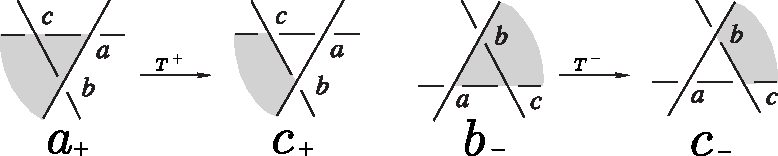
\includegraphics[width=.6\textwidth]{figs/move_iiib3.pdf}
\caption{}
\label{fig:move_iiib3}
\end{figure}

Define the map $T_u^+ : \mathcal{P}(M_u) \to \bigcup_{k\ge 1} W^+_k(\Ypm,v)$,
by  $C \mapsto u^C$. Then
\footnote{Here $\mathcal{P}(M_u)$ denotes the power set.}
\begin{equation}
\label{eq:sq_union_T}
W^+(\Ypm,v) = \bigsqcup_{u\in S^-(v)} T_u^{-} 
\end{equation}

We clime that this implies 
\begin{equation}
\label{eq:tm_as_bm_and_gm}
\pr_v \circ\: \tm^+ = \pr_v \circ\: \bm^+ \circ\: g' 
\qq\tand \pr_v \circ\: \tm^- = \pr_v \circ\: \bm^- \circ\: g''. 
\end{equation}

Let $(v_1,...,v_k) \in A^{\otimes k}$, write 
\[ (v_1,...,v_k) = (v_{I_1}, b, c, v_{I_2}, ..., b,c, v_{I_p}), \]
where $v_{I_1} \in A^{\otimes I_1}$ is a tuple containing no
consecutive $b,c$. Then if there exists $u' \in W^+_{k+1}(\Ypm,v)$, 
such that $(v_1,...,v_k) = (u'(x^k_1), ..., u'(x^{k+1}_{k}))$. By 
eq. \pref{eq:sq_union_T}, $u' = T_u^+(C)$ for some $\in S_+(v)$ and $C \in \{
1,...,k\}$. ( Actually, we most have $C = (I_1+1, I_2+2, ..., v_{I_p} + p)$ ). So 
\[ (v_{I_1}, g'(b,c),v_{I_2},...,g'(b,c),v_{I_p}) =
\qty(u(x^{k-|C|}_1),...,u(x^{k-|C|}_1)). \]
Hence for every term in $\tm^+(v_1,...,v_k)$ there is a corresponding term in
$(\bm^+ \circ g')(v_1,...,v_k)$. It is easy to check that also the converse
hold and the argument for the second equation is exactly the same.

Finally, by combining the above relations, \pref{eq:sigma_g},
\pref{eq:tm_as_bm_and_gm} and $\bm^+ = \bm^-$, as well as the fact that
$(g')^2 = \id$, we have 
%
\begin{align*}
m^- \circ g 
&= \tm^- \circ\: \sigma \circ\: g \\
&= \tm^- \circ\: g'' \circ\: g' \circ\: \sigma \\
&= \bm^- \circ\: g' \circ \sigma  \\
&= \bm^+ \circ\: g' \circ \sigma  \\
&= \tm^+ \circ \sigma   \\
&= m^+.
\end{align*}
(Note, we have suppressed the $\pr_v$ at the beginning of each line in the above
calculations. The equalities only hold in the subspace spanned by $v\ne a$.)


\subsubsection{Case $v = a$:}
When $v = a$, $g$ does no longer disepere from the LHS of equation
\pref{eq:move_iii_a_inf_rel_pr}, though, by the simplisity of $g$, it does simplify
%
\begin{align*}
LHS &:= \pr_v \circ\: \qty{ \sum_{r,s,t} g_u(\I^{\otimes r} \otimes m^+_s
\otimes \I^{\otimes t}) } \\
&= g_1 (\pr_a \circ\: m^+_n) + g_2(\pr_b, \pr_c \circ\: m^+_{n-1})
+ g_2(\pr_b \circ\: m^+_{n-1}, \pr_c).
\end{align*}

By Lemma \pref{prop:l_6.1}, we can, by decreasing $\epsilon$ if necessary,
that $H(a) > H(b), H(c)$. Hence by corollary
\pref{prop:height_sum}, 
\[ \pr_v \circ\: m^+(...,a,...) = 0, \quad\text{for } v = a,b,c. \]
Therefore the RHS of equation \pref{eq:move_iii_a_inf_rel_v}, simplifies
\[ RHS := \pr_a \circ\: m^-_n \circ\: g = \pr_a \circ\: m^-_n. \]

There are only two kinds of fragments that are relevant, the ones marked
by (1) and (2) in figure \pref{fig:move_iiib}. For $i=1,2$, let $S^{\pm,i}_k
\subset W^+_k(\Ypm, a)$ denote the set of immersions that maps a
neighbourhood of $x^k_0$ to the shaded area marked by (i). Like above we will
define pre-\Ainf-structures $\tm^{\pm, i}_n : A^{\otimes n} \to A$. 
Given $v_1,...,v_n \in \Cc$, define 
%
\begin{equation}
\tm^{\pm, i}_k(v_1, ..., v_k) = \sum_v \qty(\#_2\qty(
\tilde{\M}^v_{v_1,...,v_k}(\Ypm) \cap S^{\pm, i}_k))  v.
\end{equation}
